\chapter{Felhasználói dokumentáció}
\label{ch:user}

A következő fejezetben fogom bemutatni az alkalmazás elérését, egyes komponenseit, illetve felhasználási lehetőségeit. 

Ez a pénzügyeket rendszerező alkalmazás alapvetően magánszemélyeknek készült, személyes felhasználásra, de mivel lehetőséget nyújt csoportos használatra is, ezáltal akár egy kisebb vállalat igényeit is elláthatja.

A főbb funkciók közé tartozik, hogy bevételeket és kiadásokat lehet rögzíteni, kategóriák szerint csoportosítva, illetve kimutatásokat nézhet a felhasználó a pénzügyi szokásairól, melyeket exportálni is tudja. Az alkalmazás egyik nagy előnye, hogy nem csak egyének használhatják, hanem csoportok (például háztartások) is.


\section{Rendszerkövetelmények}

Mivel egy webes alkalmazásról van szó, ezért különleges gépigény nem szükséges. Szinte az összes böngésző támogatott.

\section{Felhasználói esetek}
Az alkalmazás felhasználói eseteit ez a bejegyzés fogja taglalni jobban, képernyőképekkel magyarázva.

\subsection{Fiók}
\begin{table}[H]
	\centering
	\begin{tabular}{ | m{0.25\textwidth} | m{0.65\textwidth} | }
		\hline
		\textbf{Funkció} & \textbf{Leírás} \\
		\hline \hline
		\emph{Bejelentkezés} & Bejelentkezés egy egyedi felhasználónévvel és egy jelszóval lehetséges. \\
		\hline
		\emph{Regisztráció} &  Regisztrálni lehet az oldalra a következő adatok megadásával: e-mail cím, felhasználónév (egyedi), teljes név, jelszó (minimum 8 karakter, legalább 1 szám, legalább 1 nagy betű, legalább 1 speciális karakter).  \\
		\hline
		\emph{Elfelejtett jelszó} & Ha a felhasználó elfelejtette a jelszavát, akkor a Bejelentkezés felületen az "Elfelejtett jelszó" hivatkozásra kattintva megjelenik egy új felület, csak egy e-mail beviteli mezővel. A rendszer küldeni fog egy egyedi tokennel ellátott linket a megadott e-mail címre (amely 30 percig érvényes), és ezen a linken tudja a felhasználó majd megadni az új jelszavát (szintén a biztonsági kritériumoknak megfelelő formában), és sikeres bejelentkezést követően már bent is lesz a fiókjában. \\
		\hline
		\emph{Kijelentkezés} & Ha a felhasználó befejezte kívánt tevékenységét, akkor a bal oldali menüsáv alján található "Logout" gomb megnyomásával tud kijelentkezni. Alapvetően 30 perc inaktivitás után "dob le" az oldal (azaz jár le az adott session). \\
		\hline
	\end{tabular}
	\caption{Fiók műveletek}
	\label{tab:account}
\end{table}

\begin{figure}[H]
	\centering
	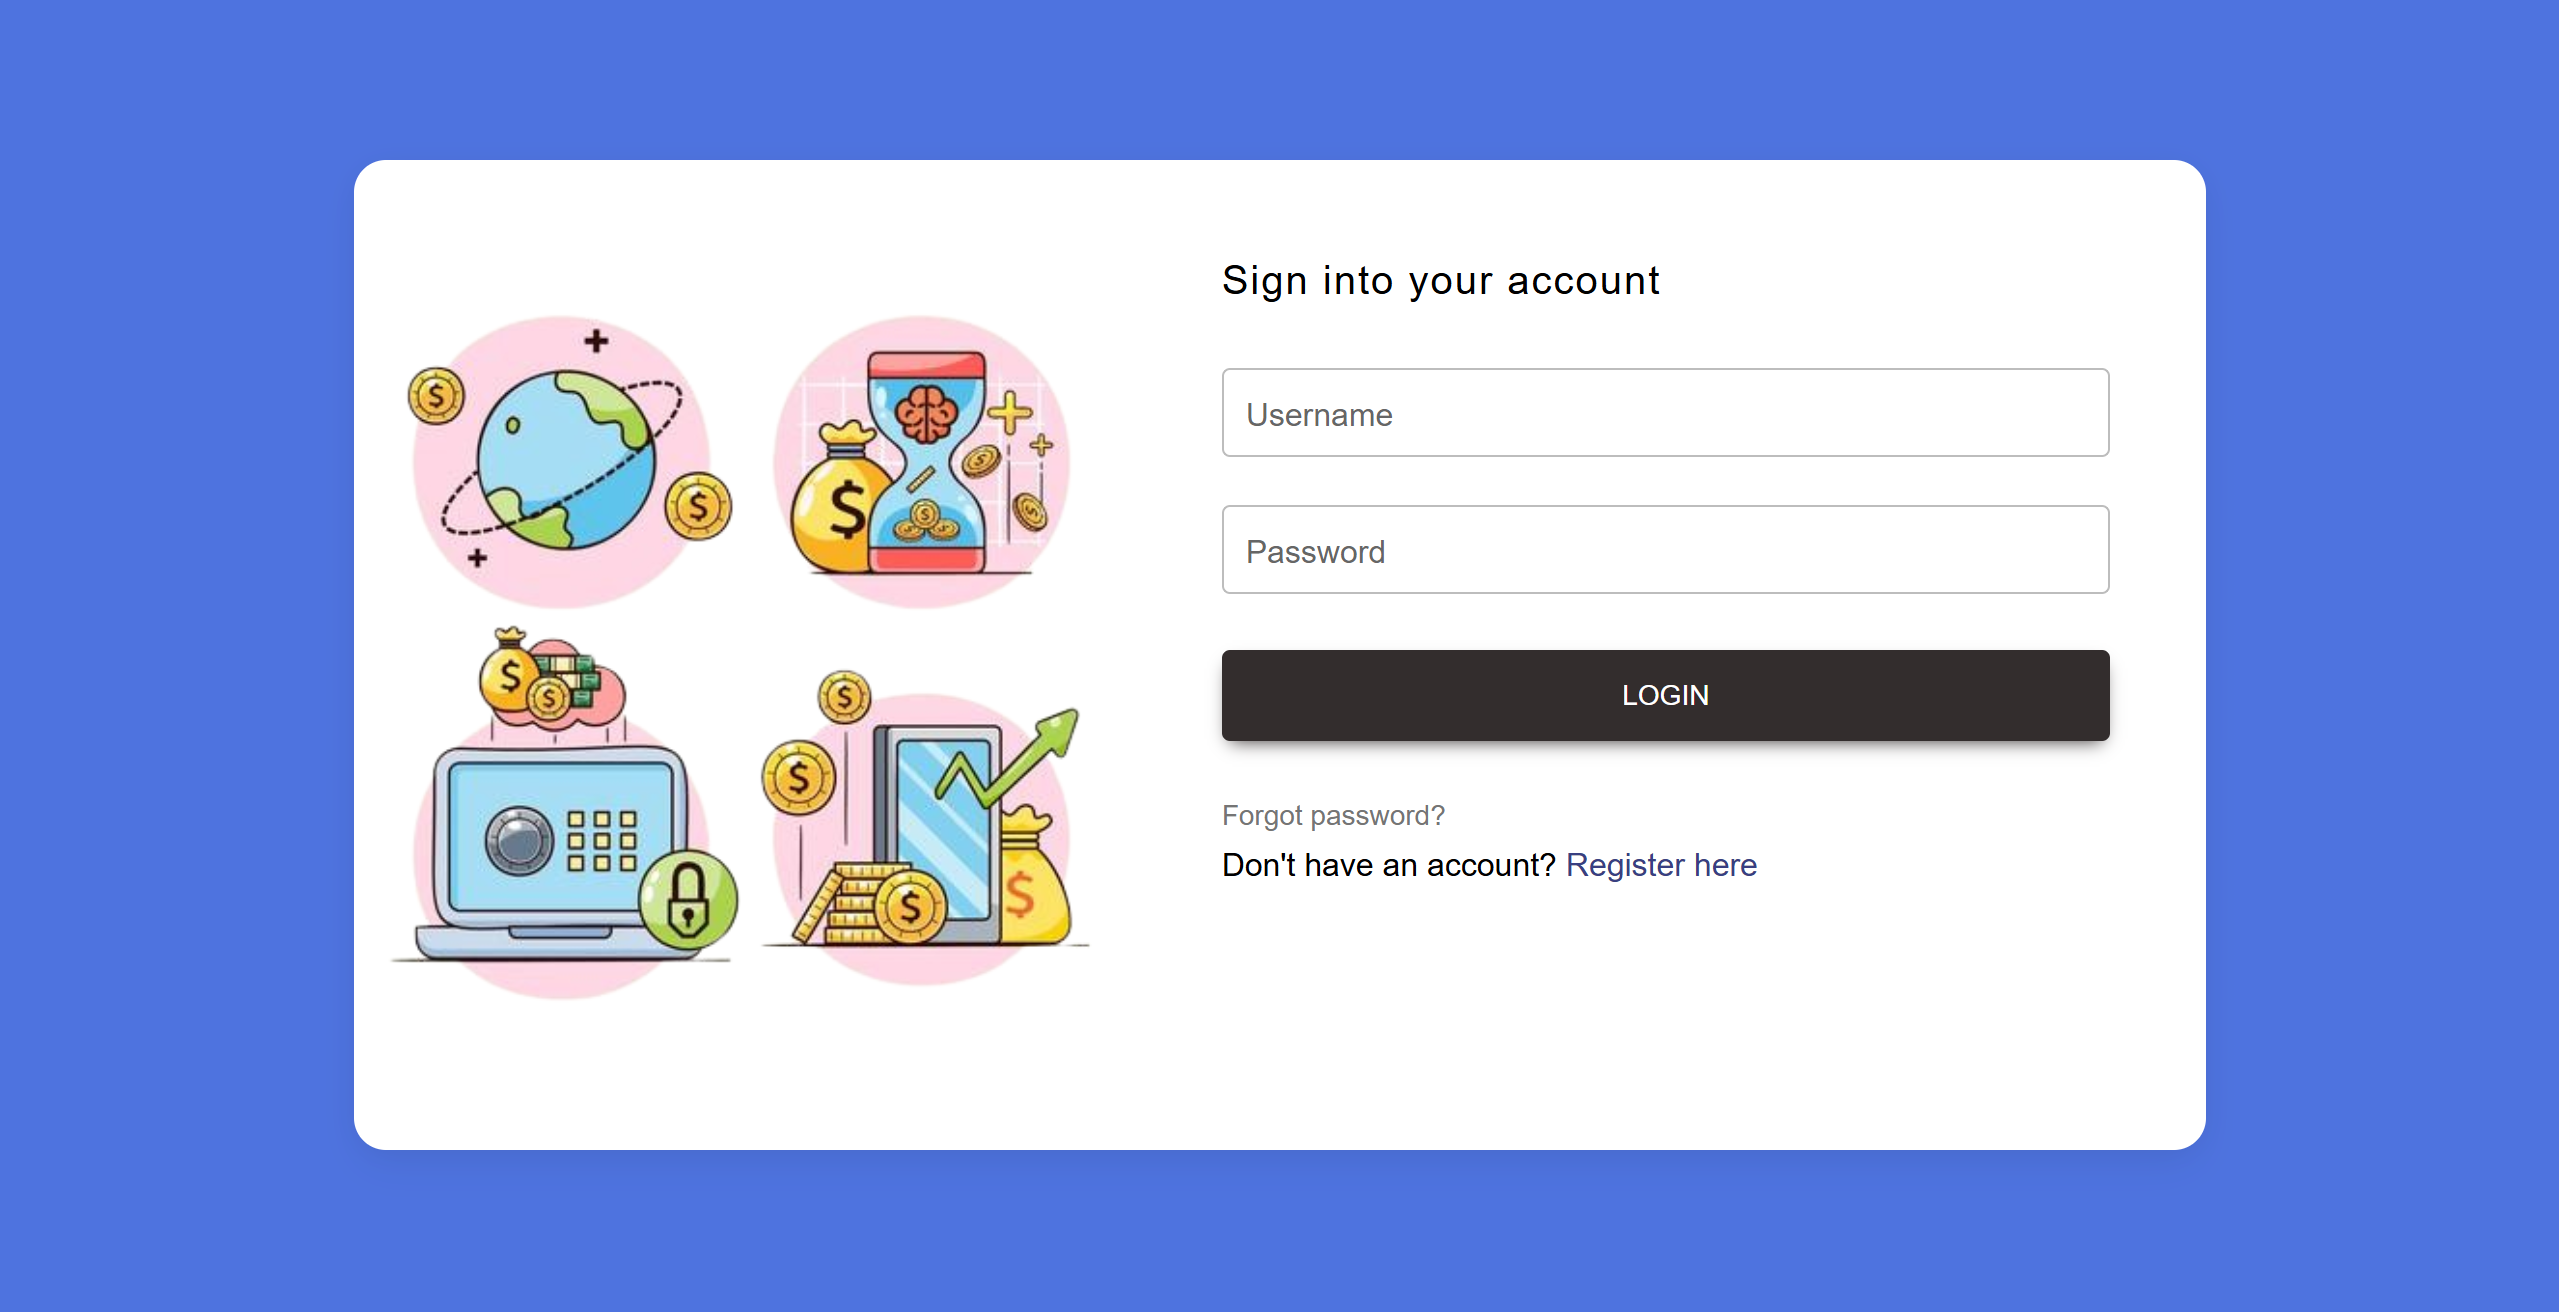
\includegraphics[height=180px]{img/login-screenshot}
	\caption{Screenshot: Bejelentkező felület}
	\label{fig:login}
\end{figure}

\subsection{Profil}
A profil oldalt a bal menüsávből érhetjük el.
\begin{table}[H]
	\centering
	\begin{tabular}{ | m{0.25\textwidth} | m{0.65\textwidth} | }
		\hline
		\textbf{Funkció} & \textbf{Leírás} \\
		\hline \hline
		\emph{Adatok megtekintése} & A regisztrációnál megadott személyes adatait a felhasználó itt tekintheti meg. \\
		\hline
		\emph{Adatok módosítása} &  A személyes adatok módosítására is itt van lehetőség, egyszerű beviteli mezőkkel lehet módosítani a felhasználónevet (egyedi), teljes nevet és e-mail címet.  \\
		\hline
		\emph{Jelszó módosítás} & Ha a felhasználó módosítani kívánja a jelszavát, akkor a "Jelszó módosítása" gombra kattintva megjelenik egy új felület, két jelszó beviteli mezővel (új jelszó, új jelszó megerősítése). Itt szintén érvényesek a korábban taglalt (2.1 táblázat) biztonsági kritériumok. Ezután sikeres bejelentkezést követően már bent is lesz a fiókjában. \\
		\hline
	\end{tabular}
	\caption{Profil oldal}
	\label{tab:profile}
\end{table}

\begin{figure}[H]
	\centering
	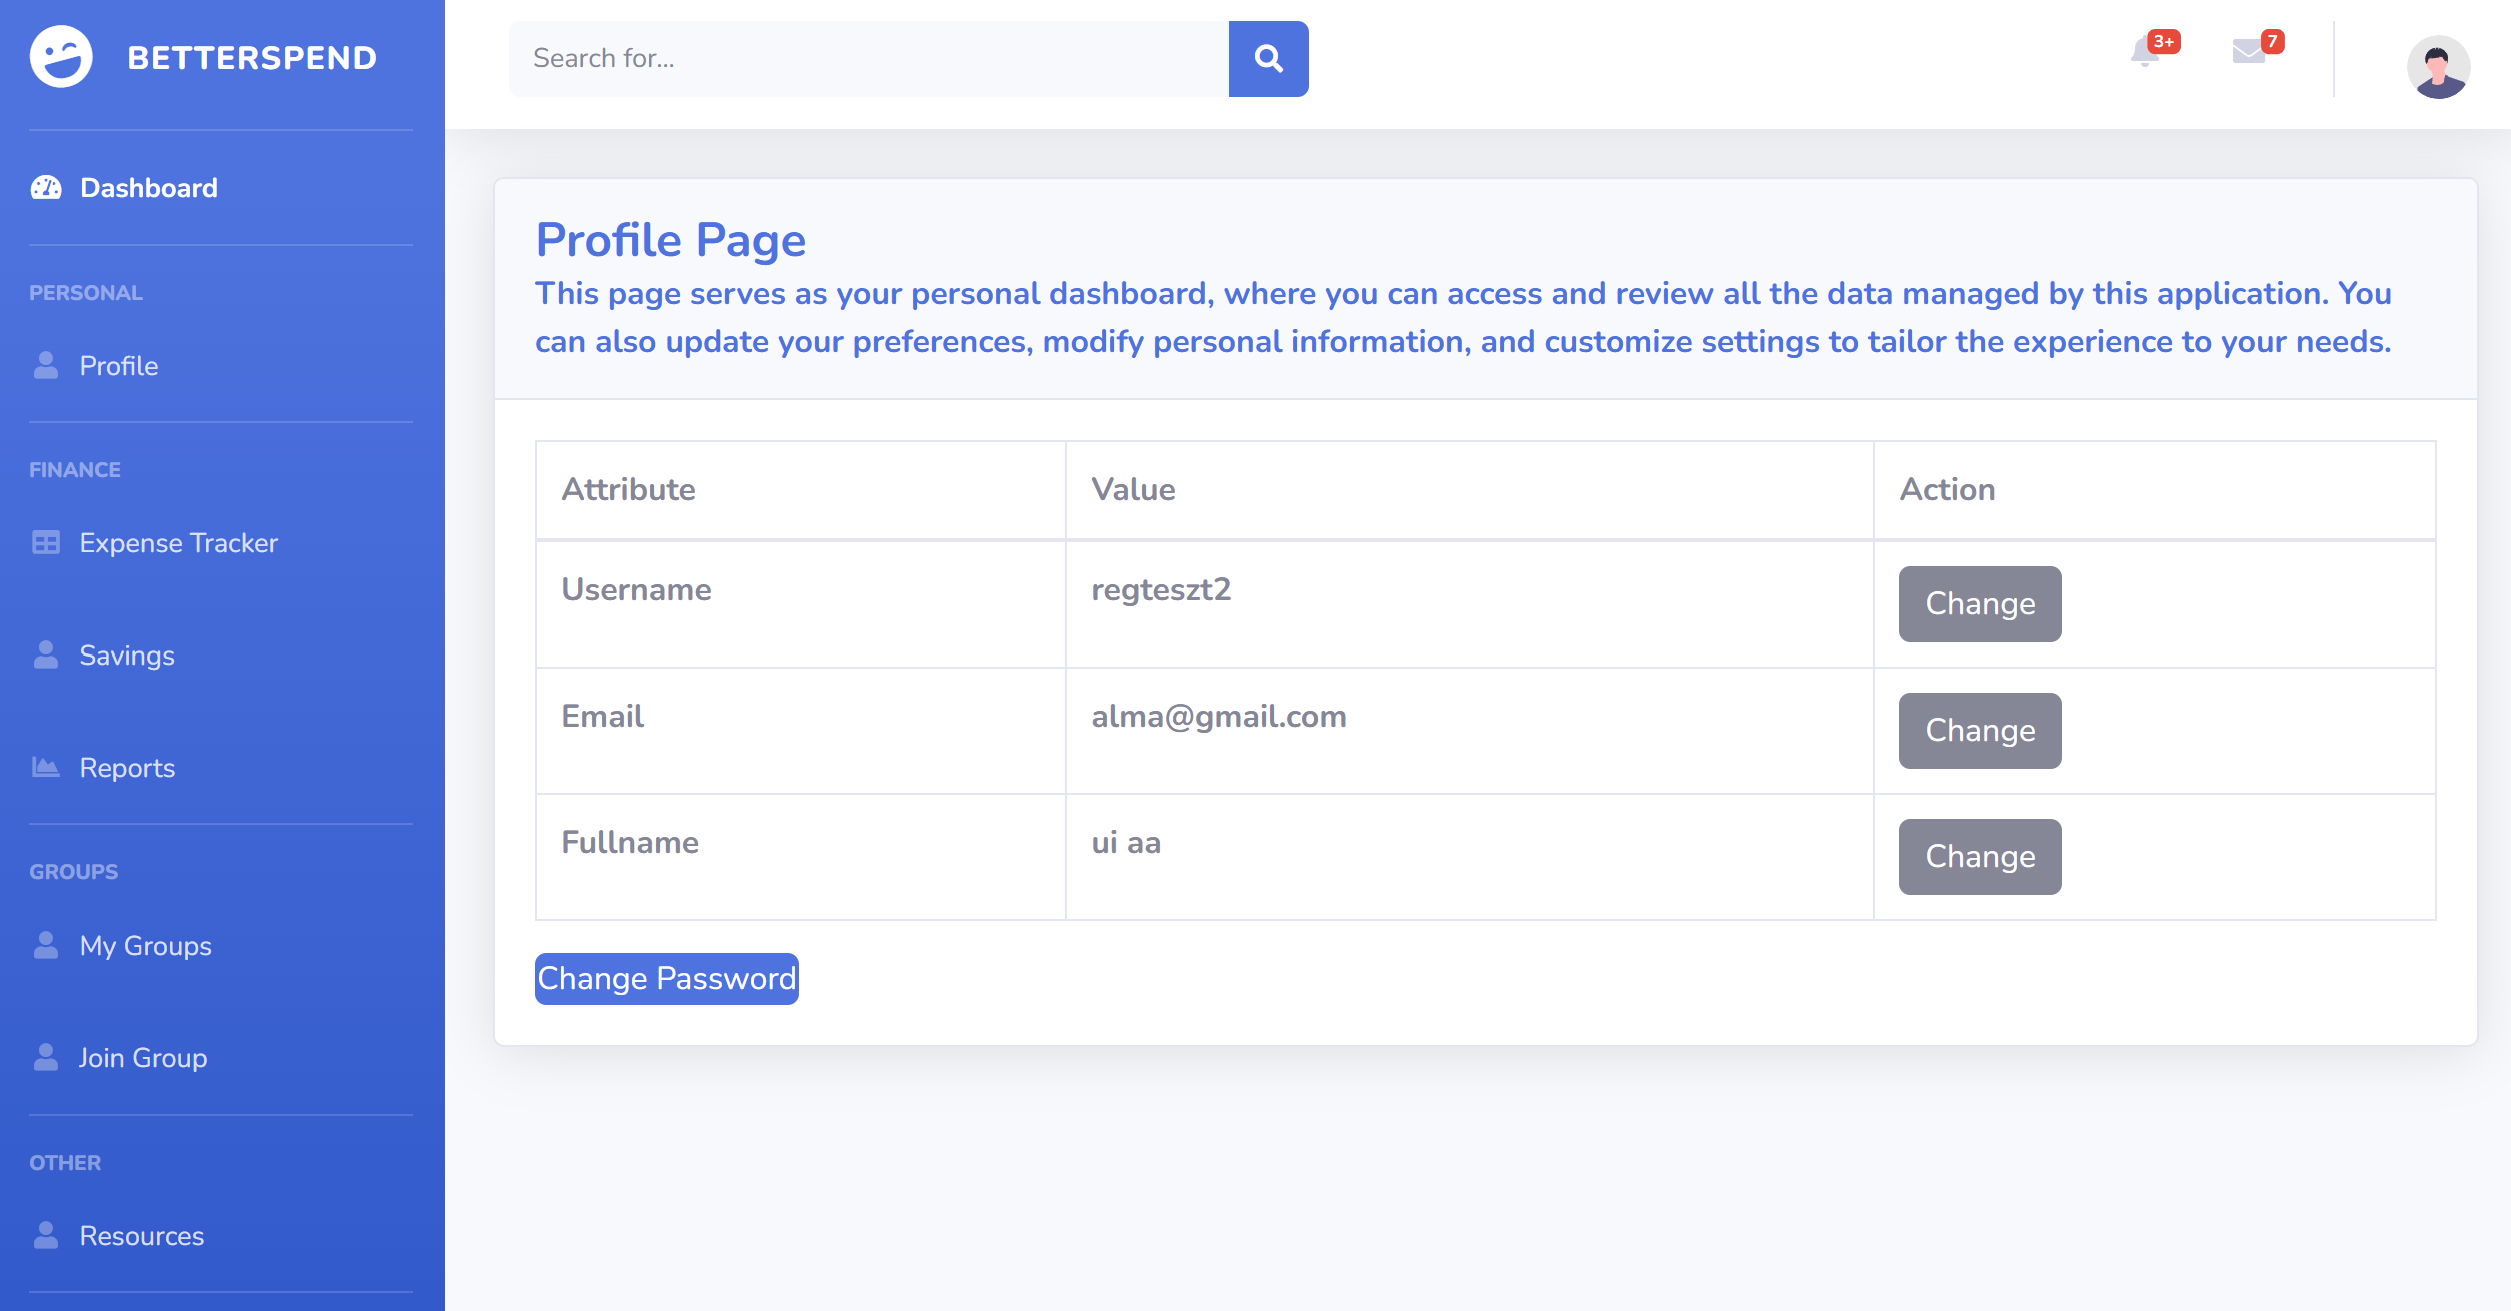
\includegraphics[height=190px]{img/profile-screenshot}
	\caption{Screenshot: Profil felület}
	\label{fig:profile}
\end{figure}

\subsection{Pénzügyek}
A pénzügyeket kezelő oldalakat a bal menüsávből érhetjük el. Ezen a főmenüponton belül is 3 almenüpont lett kialakítva: 
\begin{itemize}
	\item Expense Tracker (Bevételek és kiadások vezetése, és előzmények megtekintése)
	\item Savings (Megtakarítások megtekintése és kezelése)
	\item Reports (Kimutatások megtekintése, személyre szabása és exportálása)
\end{itemize}

\begin{table}[H]
	\centering
	\begin{tabular}{ | m{0.25\textwidth} | m{0.65\textwidth} | }
		\hline
		\textbf{Funkció} & \textbf{Leírás} \\
		\hline \hline
		\emph{Kiadás/bevétel rögzítése} & Külön dobozokban lehet rögzíteni a kiadásokat, és a bevételeket. Egyszerre egyet lehet bevinni, melynek adni kell egy összeget, egy leírást, opcionálisan lehet kategóriát is megadni. \\
		\hline
		\emph{Előzmények} &  A költési és bevételi előzményeket is itt lehet megtekinteni.  \\
		\hline
	\end{tabular}
	\caption{Expense Tracker oldal}
	\label{tab:expense-tracker}
\end{table}

\begin{figure}[H]
	\centering
	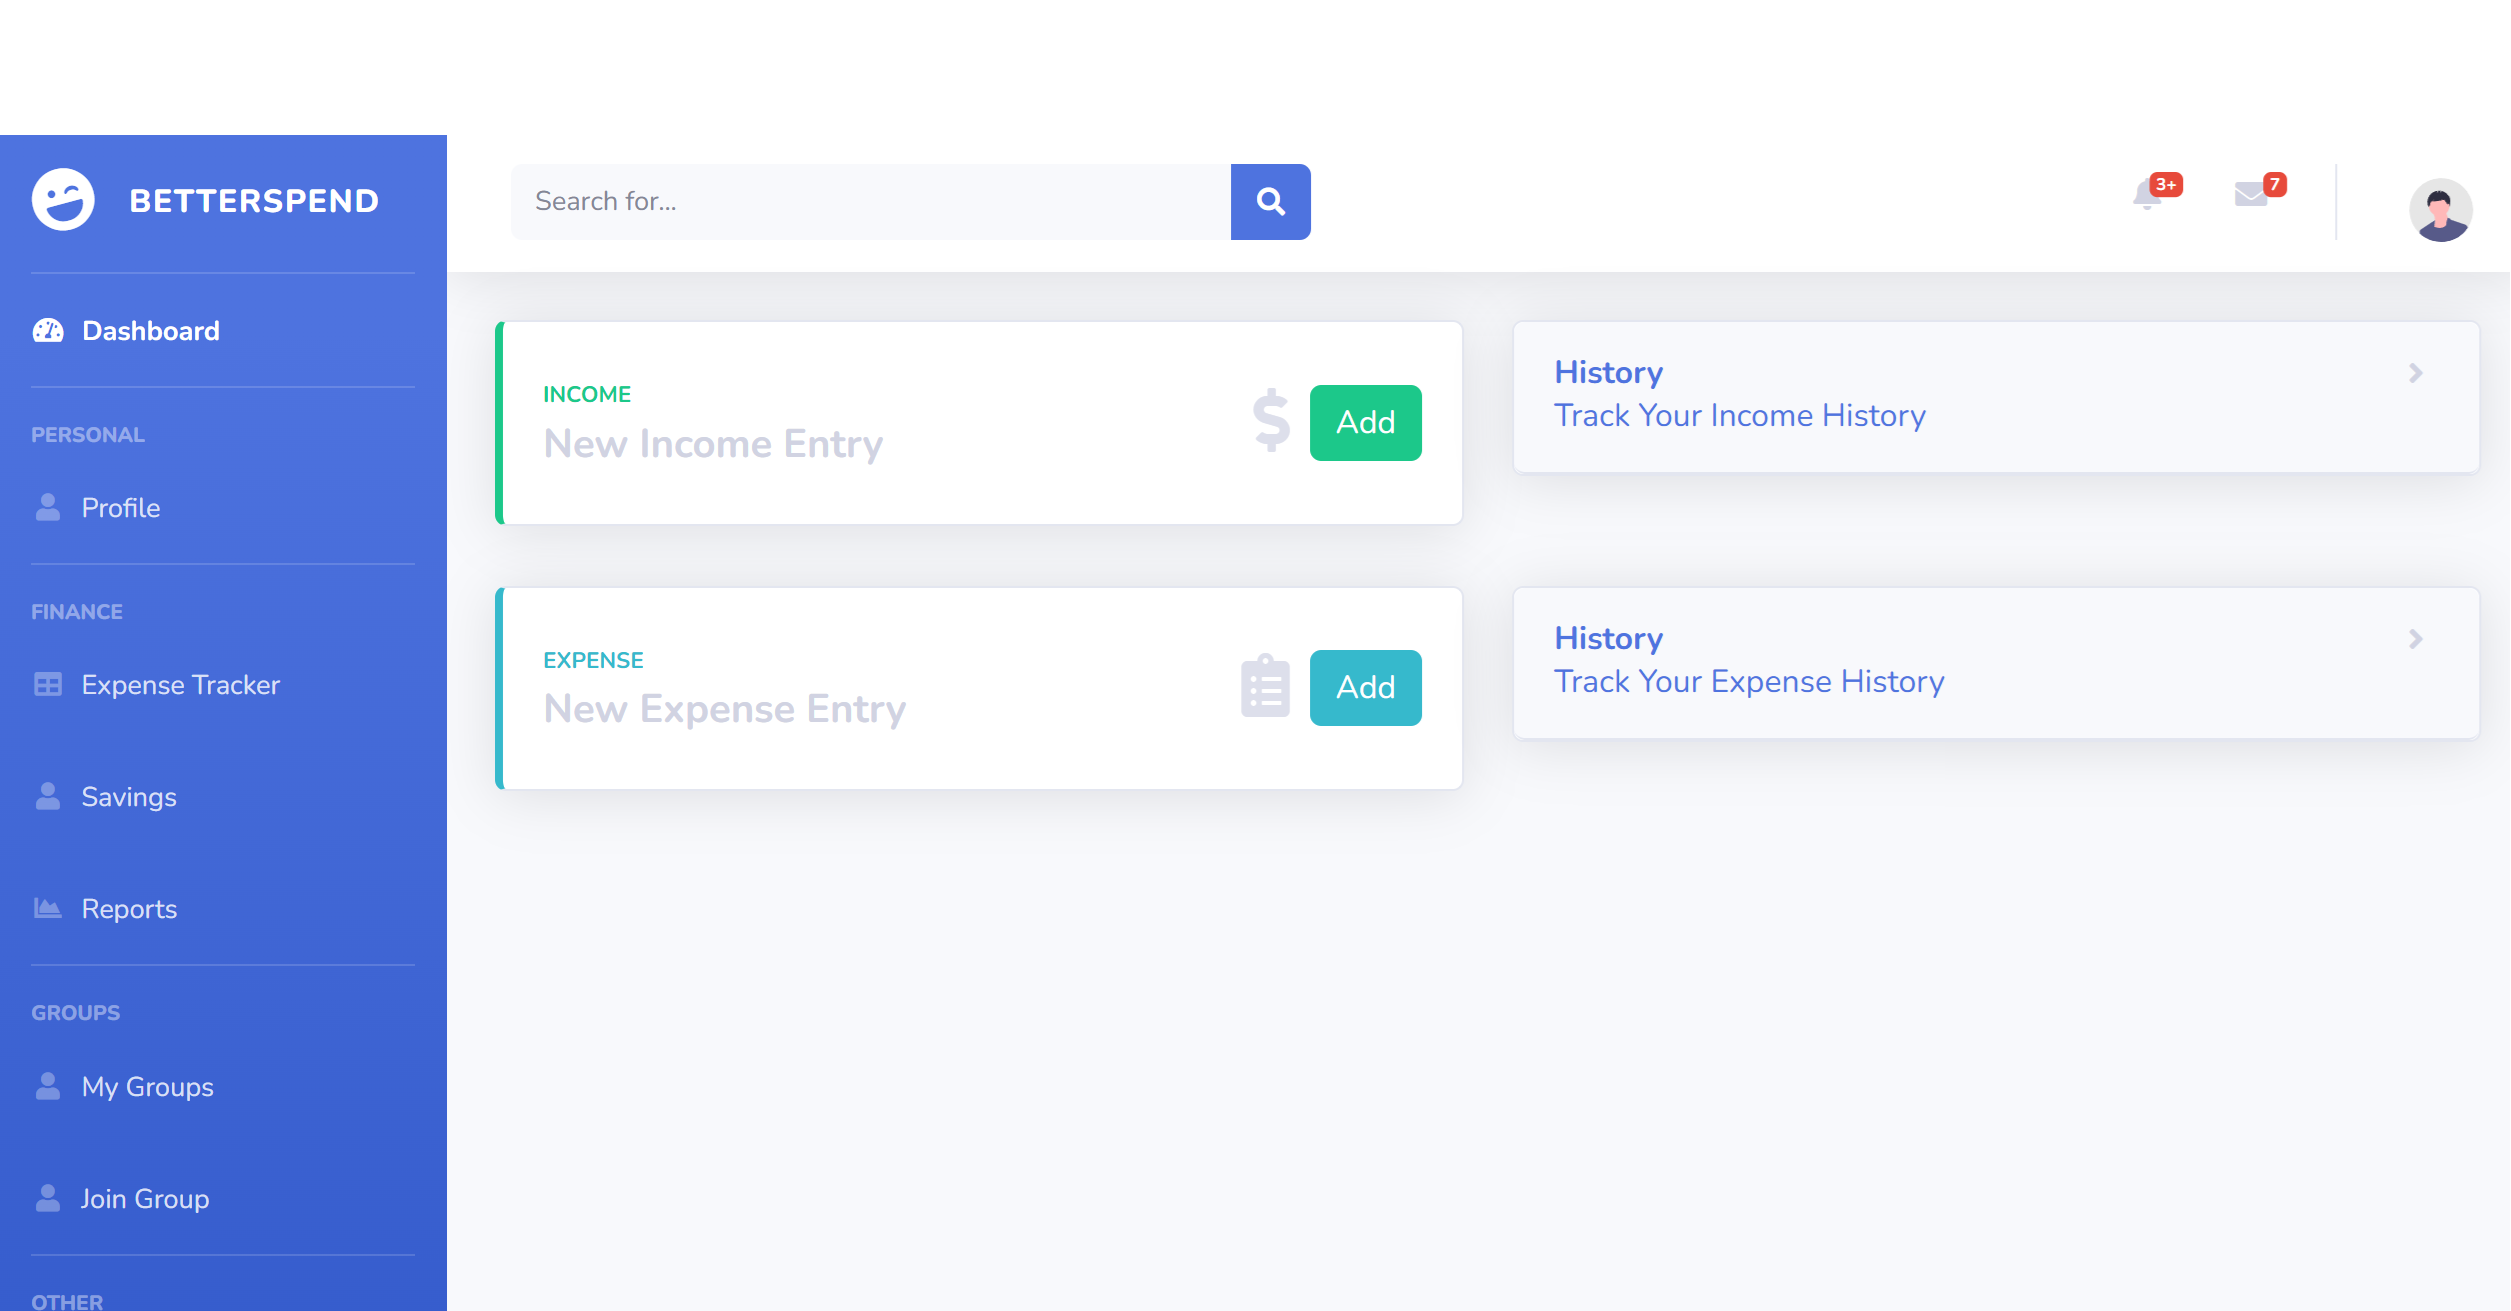
\includegraphics[height=190px]{img/expense-tracker-screenshot}
	\caption{Screenshot: Expense Tracker felület}
	\label{fig:expense-tracker}
\end{figure}

\begin{table}[H]
	\centering
	\begin{tabular}{ | m{0.25\textwidth} | m{0.65\textwidth} | }
		\hline
		\textbf{Funkció} & \textbf{Leírás} \\
		\hline \hline
		\emph{-} & - \\
		\hline
	\end{tabular}
	\caption{Savings oldal}
	\label{tab:savings}
\end{table}

\begin{table}[H]
	\centering
	\begin{tabular}{ | m{0.25\textwidth} | m{0.65\textwidth} | }
		\hline
		\textbf{Funkció} & \textbf{Leírás} \\
		\hline \hline
		\emph{-} & - \\
		\hline
	\end{tabular}
	\caption{Reports oldal}
	\label{tab:reports}
\end{table}

\subsection{Csoportok}
-